%TODO: CORREGIR COMANDOS PARA QUE SE VEAN CON VERB
%TODO: INTENTAR QUITAR LA MORRAYA QUE NO SIRVA
%TODO: INTENTAR NO REPETIR TANTAS COSAS EN EL EJERCICIO 3
%TODO: REVISAR DOCUMENTO PARA FALLOS ORTOGRAFICOS/GRAMATICALES
\documentclass{article}
\usepackage[utf8]{inputenc}
\usepackage[spanish]{babel}
\usepackage{graphicx, graphics, float, hyperref}
\usepackage{listings}
\usepackage[a4paper, total={6in, 10in}]{geometry}

\title{SSO Práctica 2 Sesión 1}
\author{Andrés Merlo Trujillo}
\date{}
\hypersetup{
    colorlinks=true,
    linkcolor=black,
}

\begin{document}

\maketitle

\tableofcontents

\newpage
%\addcontentsline{toc}{section}{Ejercicio 1}
%\section*{Ejercicio 1}
%\begin{figure}[H]
%    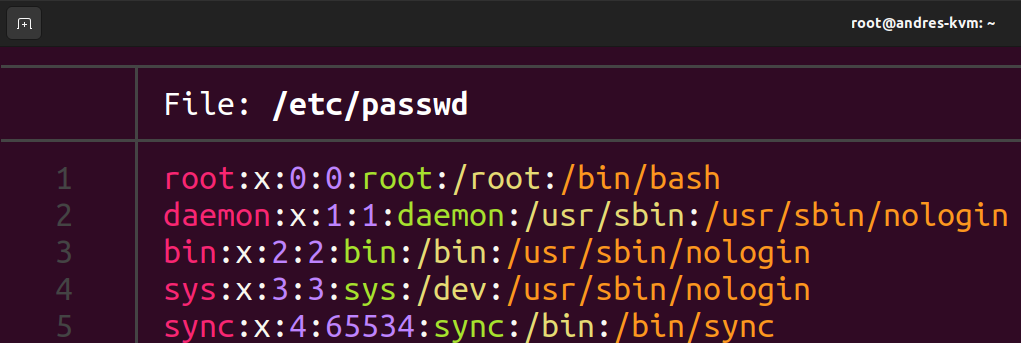
\includegraphics[width=\textwidth]{imagenes/passwdfile.png}
%    \caption{Ejemplo de entradas en el archivo.}
%\end{figure}

\addcontentsline{toc}{section}{Ejercicio 1}
\section*{Ejercicio 1}

Para ello voy a crear los siguientes programas:

%foto programa C++

%foto programa C

Y voy a usar las siguientes ordenes para compilarlos:

\verb|g++ -o salidaCPP holaMundo.cpp|
\verb|gcc -o salidaC holaMundo.c|


\addcontentsline{toc}{subsection}{Apartado A}
\subsection*{Apartado A}
A continuacion explicaré que contiene cada seccion, para obtener informacion se puede usar la orden \verb|man 5 elf|:

\begin{itemize}
    \item \textbf{.interp}: Esta seccion almacena la ruta del interprete del programa. Si el archvo tiene un segmento que incluye esta seccion, los atributos de la seccion tendran el bit SHF\_ALLOC. La seccion es de tipo SHT\_PROGBITS.
    
    \item \textbf{.got}: Esta seccion almacena la tabla de desplazamientos global (Global Offset Table). Es de tipo SH\_PROGBITS y sus atributos son especificos del procesador. 
    
    \item \textbf{.got.plt}: Esta seccion almacena la tabla de vinculacion de procedimientos (Procedure Linkage Table). Es de tipo SH\_PROGBITS y sus atributos son especificos del procesador. Sirve para obtener las direcciones a funciones para posteriormente poder ser llamadas.
\end{itemize}


\addcontentsline{toc}{subsection}{Apartado B}
\subsection*{Apartado B}

Ejecutando la orden \verb|readelf -S ejecutable| podemos obtener las secciones que componen el programa.

%foto de cpp con readelf

%foto de c con readelf

Ahora, para mostrar por terminal la diferencia de los archivos a color se puede usar la orden \verb|icdiff archivo1 archivo2|.

%foto de icdiff (quizas haya que cortarlas)

Como se puede ver, en la primera linea, el offset es distinto, siendo mas alto en el programa escrito en C++. Ademas, se puede ver que algunas secciones del programa escrito en C++ son ligeramente mas grandes que la version en C. Las secciones afectadas son: .gun.hash, .dynsym, .dynstr, .gun.version, .rela.dyn, .rela.plt, .plt, .plt.sec, .text, .eh\_frame\_hdr, .eh\_frame, .init\_array, .fini\_array, .dynamic, .got, .bss, .symtab, y .strtab.

Por ultimo, tambien se puede ver que el desplazamiento (offset) y las direcciones de memoria de estas secciones varia entre una version y otra.


\bigskip

Las secciones .ctors y .dtors contienen lo siguiente:

\begin{itemize}
    \item \textbf{.ctors}: Esta seccion almacena punteros inicializados a las funciones del constructor de C++ (constructores de las clases).
    \item \textbf{.dtors}: Esta seccion almacena punteros inicializados a las funciones del destructor de C++ (destructores de las clases).
\end{itemize}
\end{document}
